\documentclass[10pt]{article}
\usepackage[a4paper,margin=0.55in]{geometry}
\usepackage{amsmath,amsfonts,amssymb}
\usepackage{booktabs}
\usepackage{graphicx}
\usepackage{hyperref}
\usepackage{siunitx}
\usepackage[font=footnotesize,labelfont=bf]{caption}
\usepackage[section]{placeins}
\graphicspath{{tex_images/}}
\setlength{\parindent}{0pt}
\setlength{\parskip}{3pt}
\setlength{\textfloatsep}{8pt}
\setlength{\floatsep}{6pt}
\setlength{\intextsep}{6pt}
\emergencystretch=2em
\renewcommand{\arraystretch}{0.9}

\title{Parametric and Kernel Models for Chiral Line Fields}
\author{Rishabh Kumar}
\date{\today}

\begin{document}
\maketitle

\begin{abstract}
The analysis compares a low-dimensional parametric spiral family with two non-parametric kernel-regression frameworks, Nadaraya--Watson (NW) local smoothing and Gaussian-process/kernel-ridge regression (GP/KRR).  The two datasets have different observation structures: the Gabor data provide samples of a director/vector field encoded by local pitch relative to the radial frame, while the optical SEM data provide unoriented line segments.  Both are analyzed through axial angles, so directions separated by $\pi$ are equivalent.  Model selection is based on held-out axial RSS.  The central empirical finding is that the RBF--von-Mises kernel captures the relevant polar geometry; GP/KRR can lower held-out RSS for smooth positive kernels, but NW remains the more conservative local descriptive smoother when fitted streamlines indicate possible overfitting.
\end{abstract}

\section{Shared Observation Model}
The two data sources differ before modelling.  In the Gabor data, a sampled director/vector field is reduced to a local pitch angle $\alpha_i'$; the radial frame supplies the missing global rotation.  In the optical SEM data, the input is an unoriented line segment, and only the axis of the segment is observed.  Thus the raw observations may be directed vectors, directors, or line fields.  For a common comparison criterion, each observation is projected to an axial angle $\hat\alpha_i$, where $\hat\alpha_i$ and $\hat\alpha_i+\pi$ are equivalent.  Following the standard treatment of axial data in directional statistics \cite{mardia2000}, the response is embedded as
\begin{equation}
  u_i=(\cos 2\hat\alpha_i,\sin 2\hat\alpha_i)\in\mathbb R^2.
  \label{eq:embedding}
\end{equation}
For a fitted angle $\alpha_{\mathcal M}(z_i)$, the axial residual is
\begin{equation}
  \Delta_i^{\rm ax}(\mathcal M)
  =
  \frac12\operatorname{atan2}\!\left(
    \sin 2\{\hat\alpha_i-\alpha_{\mathcal M}(z_i)\},
    \cos 2\{\hat\alpha_i-\alpha_{\mathcal M}(z_i)\}
  \right).
  \label{eq:axial-residual}
\end{equation}
Held-out error is reported as fold-averaged per-observation RSS,
\begin{equation}
  {\rm RSS}_{\rm test}(\mathcal M)=
  \frac1K\sum_{k=1}^K\frac1{|I_k|}
  \sum_{i\in I_k}\{\Delta_i^{\rm ax}(\mathcal M_{-k})\}^2.
  \label{eq:test-rss}
\end{equation}
This axial projection gives the common observation model used for both parametric and non-parametric fits.  The only difference is the mean field $\alpha_{\mathcal M}(z)$ used to predict the projected angle.

The angles are noisy measurements of an underlying field, not deterministic targets.  A local vector-noise model is
\begin{equation}
  W_i=F_{\theta_0}(Z_i)+\varepsilon_i,\qquad
  \varepsilon_i\sim N(0,\sigma^2I_2),
  \qquad
  \hat\alpha_i=\operatorname{atan2}(W_{i,2},W_{i,1}).
  \label{eq:vector-noise}
\end{equation}
Writing $\alpha_{\theta_0}(z)=\operatorname{atan2}\{F_{\theta_0,2}(z),F_{\theta_0,1}(z)\}$ and $\rho_{\theta_0}(z)=\|F_{\theta_0}(z)\|_2$, the delta method \cite{vanDerVaart2000} gives the local approximation
\begin{equation}
  \hat\alpha_i
  \approx
  \alpha_{\theta_0}(Z_i)+\eta_i,
  \qquad
  {\rm Var}(\eta_i)\approx\frac{\sigma^2}{\rho_{\theta_0}(Z_i)^2}.
  \label{eq:heteroskedastic-angle}
\end{equation}
Thus angle noise is heteroskedastic: weak local vector magnitude produces noisier angle measurements.  The present experiments use unweighted axial RSS, so the reported model comparisons should be read as reconstruction-risk comparisons rather than full likelihood fits for \eqref{eq:heteroskedastic-angle}.

For the optical SEM data, $z_i$ is the midpoint of an image-derived line segment and $\hat\alpha_i=\operatorname{atan2}\{-(y_{2i}-y_{1i}),x_{2i}-x_{1i}\}$ after flipping the image $y$-axis into mathematical coordinates.  For the Gabor data, the observed angle is a pitch angle $\alpha_i'$ relative to the radial frame, so the global axial field angle is
\begin{equation}
  \phi_i=\theta_i+\alpha_i',
  \qquad
  \theta_i=\operatorname{atan2}(y_i,x_i).
  \label{eq:gabor-angle}
\end{equation}
The Gabor regressions therefore fit $\alpha'(z)$ and reconstruct $\phi(z)=\theta(z)+\alpha'(z)$.

\begin{figure}[!htbp]
\centering
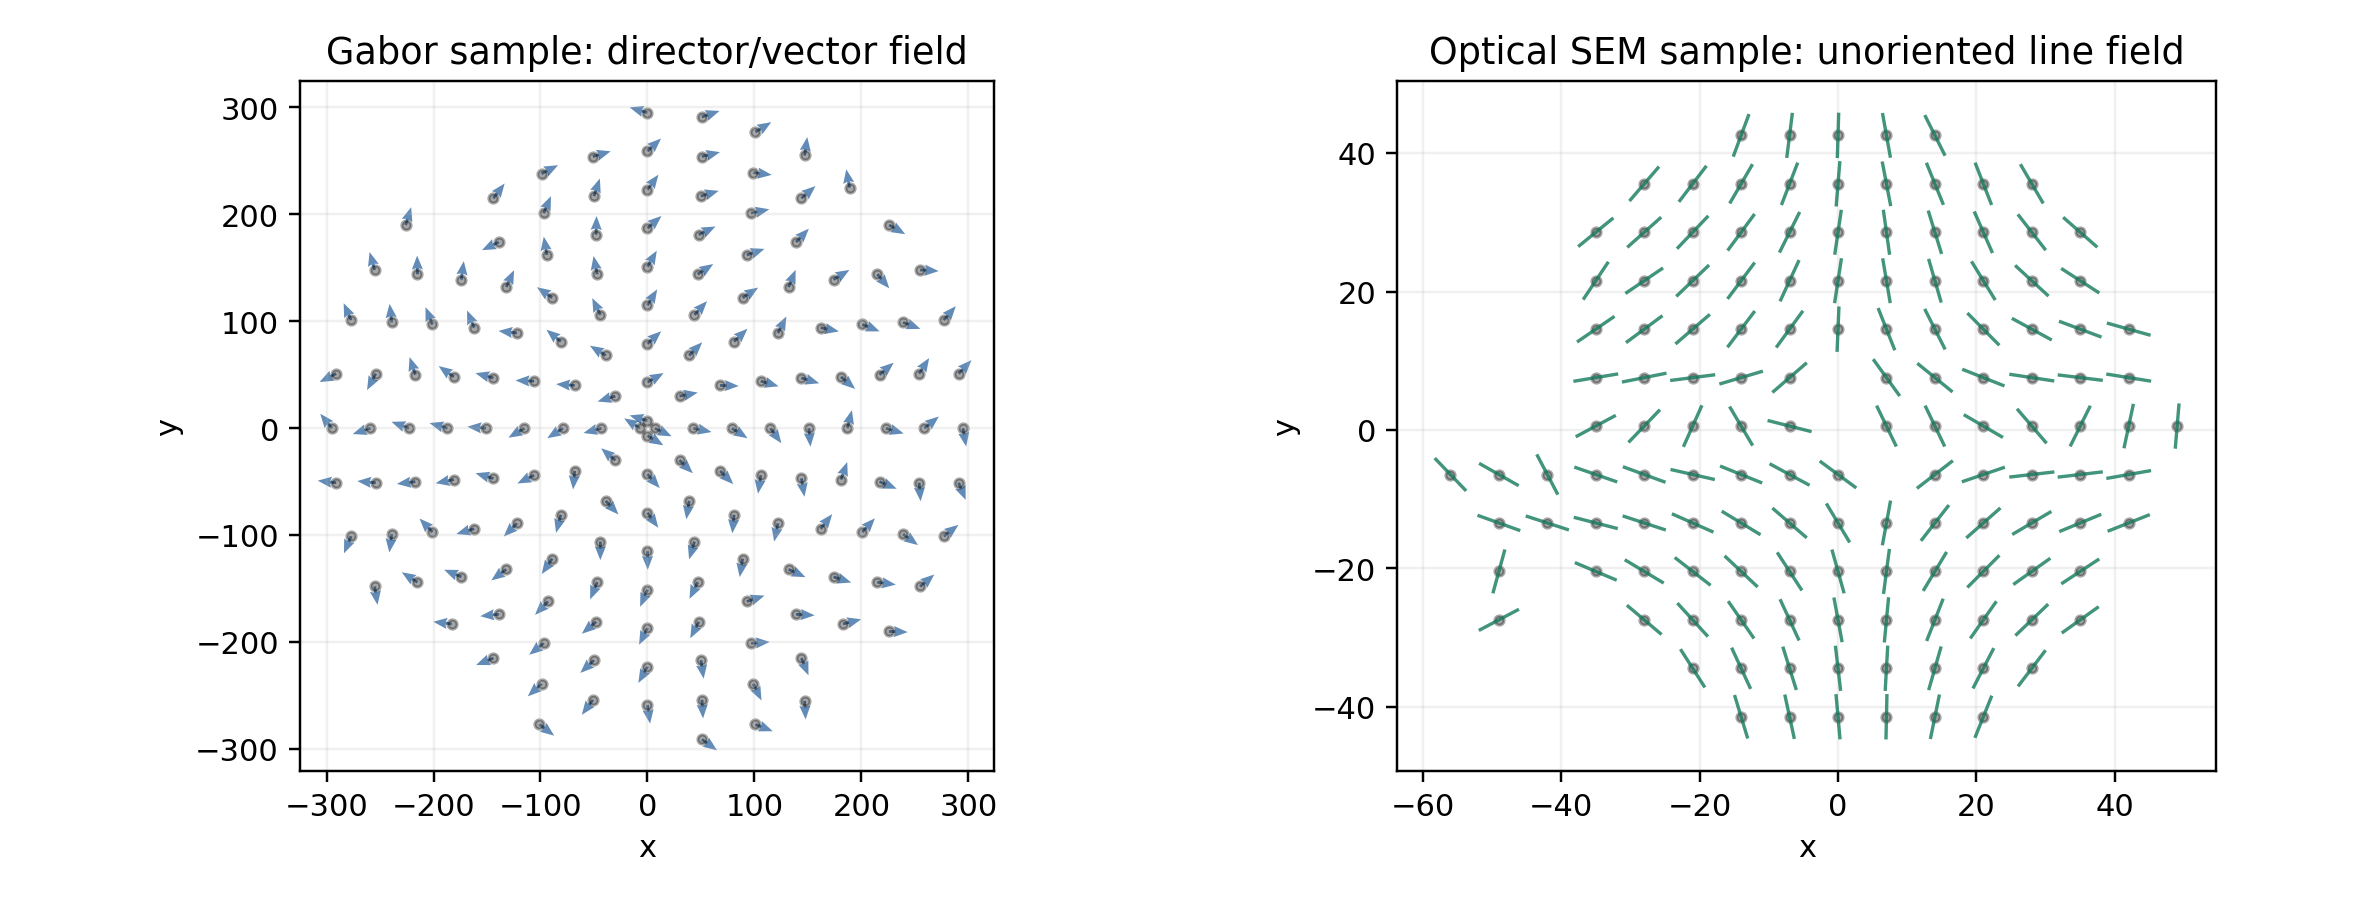
\includegraphics[width=0.88\linewidth]{observed_data_examples.png}
\caption{Representative observed data.  Left: a Gabor director/vector-field sample, where the measured pitch is interpreted relative to the radial frame.  Right: an optical SEM sample after converting image segments to unoriented line-field observations.}
\label{fig:observed-data}
\end{figure}

\section{Models}
Equation~\eqref{eq:heteroskedastic-angle} gives the statistical template for all model classes:
\[
  \hat\alpha_i = m(z_i)+\eta_i \quad {\rm mod}\ \pi,
\]
where $m$ is the unknown mean axial field angle after the common projection and $\eta_i$ is angle noise induced by measurement noise in the underlying vector, director, or segment estimate.  Model selection is therefore a question about the function class used for $m$.  The parametric spiral family restricts $m$ to a low-dimensional spiral form; NW and GP/KRR replace that form by a kernel-based non-parametric mean estimator.

\paragraph{Potential-gradient parametric spirals.}
After centering coordinates, let $r_i=\|z_i\|_2$ and $\theta_i=\operatorname{atan2}(y_i,x_i)$.  The parametric family is the line direction induced by the potential-gradient field
\[
  V_{p,A,b}(r,\theta)=A g_p(r)-b\theta,\qquad
  g_p(r)=
  \begin{cases}
    \log r, & p=0,\\
    r^p/p, & p\ne0,
  \end{cases}
\]
for which
\[
  \nabla V_{p,A,b}(r,\theta)=A r^{p-1}\mathbf e_r-\frac{b}{r}\mathbf e_\theta .
\]
Only the ratio $b/A$ is identifiable from angles.  Writing $A=\cos\gamma$ and $b=\sin\gamma$, the mean angle used in the implementation is
\begin{equation}
  m_{p,\gamma}(z_i)=
  \theta_i+\operatorname{atan2}\{-\sin(\gamma),\cos(\gamma)r_i^p\}
  \quad {\rm mod}\ \pi .
  \label{eq:parametric}
\end{equation}
The stochastic observation model is then $\hat\alpha_i=m_{p,\gamma}(z_i)+\eta_i$ modulo $\pi$.  The fixed families are $p=0,1,2$; the continuous family estimates $p\in(-1,3)$ as part of the mean function.  For fixed $p$, $\gamma\in[-\pi,\pi]$ is fit by a deterministic grid followed by L-BFGS-B refinement.  The implementation minimizes empirical axial RSS, which is the corresponding least-squares or quasi-likelihood criterion under approximately homoskedastic angle noise.  Thus the parametric model is not noise-free; only its mean function is deterministic.

\paragraph{Nadaraya--Watson local regression.}
The NW fit treats the doubled-angle response as a noisy non-parametric regression observation,
\[
  u_i=\mu(z_i)+\xi_i,\qquad
  \mathbb E(\xi_i\mid z_i)=0,\qquad
  \mu(z)=(\cos 2m(z),\sin 2m(z)).
\]
No parametric form is imposed on $m$ or $\mu$.  The kernel enters only through the local weights
\[
  w_i(z)=\frac{K_\eta(z,z_i)}{\sum_j K_\eta(z,z_j)}.
\]
Thus $K_\eta(z,z_i)$ is not a covariance in the NW model; it is a window function that determines how much observation $i$ contributes to the estimate at $z$.  A small bandwidth gives nonzero weight only to nearby observations, while a large bandwidth makes the estimator closer to a global average.  Following Nadaraya and Watson \cite{nadaraya1964,watson1964}, at each target point $z$ the estimator is the local constant conditional mean, equivalently the solution of
\[
  \hat u_{\rm NW}(z)=
  \arg\min_{v\in\mathbb R^2}\sum_i K_\eta(z,z_i)\|u_i-v\|_2^2,
\]
which has the closed form
\begin{equation}
  \hat u_{\rm NW}(z)=
  \frac{\sum_i K_\eta(z,z_i)u_i}{\sum_i K_\eta(z,z_i)},
  \qquad
  \hat\alpha_{\rm NW}(z)=\frac12\operatorname{atan2}\{\hat u_2(z),\hat u_1(z)\}.
  \label{eq:nw}
\end{equation}
For the Gabor data, $u_i=(\cos 2\alpha_i',\sin 2\alpha_i')$ and the fitted pitch is added back to $\theta(z)$.  This is a local conditional-mean model rather than a full likelihood: it requires a useful nonnegative weighting rule with a nonzero denominator.  Positive definiteness is required only if the same kernel is to be used as a GP/KRR covariance.

\paragraph{GP/KRR regression.}
GP/KRR uses a stronger probabilistic model for the same embedded responses.  For output coordinate $j=1,2$,
\[
  f_j\sim{\rm GP}(0,K_\eta),\qquad
  U_{ij}=f_j(z_i)+\varepsilon_{ij},\qquad
  \varepsilon_{ij}\stackrel{\rm iid}{\sim}N(0,\sigma_n^2),
\]
with the two coordinates treated as conditionally independent given the latent functions.  The posterior mean is
\begin{equation}
  \hat u_{\rm GP}(z)=K_\eta(z,Z)\{K_\eta(Z,Z)+\sigma_n^2I\}^{-1}U,
  \label{eq:gpkrr}
\end{equation}
where $U$ has rows $u_i$.  The same expression is kernel ridge regression with squared loss and Tikhonov regularization.  Universality of the Gaussian RBF kernel is relevant mainly to this RKHS/GP viewpoint: it says the RKHS is a flexible approximation class on compact sets \cite{steinwart2001}.  It does not imply finite-sample superiority, and it is not needed to justify NW as a local smoother.

\paragraph{Kernels and sweeps.}
The three kernels are
\begin{align}
  K_{\rm RBF}(z,z';h)&=\exp[-d(z,z')^2/(2h^2)],\\
  K_{\rm unif}(z,z';h)&=\mathbf 1\{d(z,z')\le h\},\\
  K_{\rm mult}(z,z';h,\kappa)&=
  \exp[-d(z,z')^2/(2h^2)]\exp[\kappa\cos\{\vartheta(z)-\vartheta(z')\}].
\end{align}
For Gabor pitch smoothing, $d(z,z')=|\|z\|-\|z'\||$; for optical SEM smoothing, $d(z,z')=\|z-z'\|_2$.  To keep the Gabor model comparison on one scale, the reported Gabor table uses a single matched 20-fold protocol for the parametric, NW, and GP/KRR rows.  Its bandwidth candidates are
\[
  h_j=\exp\!\left\{\log(1)+j\frac{\log(1500)-\log(1)}{13}\right\},
  \qquad j=0,\ldots,13,
\]
i.e. 14 positive values from 1 to 1500 with a constant multiplicative ratio.  The RBF and uniform kernels sweep only these 14 bandwidths.  The multiplicative kernel crosses this bandwidth grid with
\[
  \kappa\in\{0,0.5,1,2,4,8,16,32,64\}.
\]
Thus the multiplicative kernel uses $14\times9=126$ bandwidth--$\kappa$ pairs per Gabor dataset.  For the matched optical SEM comparison, the bandwidth candidates are the eight values
\[
  h_j=\exp\!\left\{\log(1)+j\frac{\log(220)-\log(1)}{7}\right\},
  \qquad j=0,\ldots,7,
\]
and the multiplicative kernel uses $\kappa\in\{0,0.5,1,2,4,8,16,32\}$.  In both matched comparisons, the GP/KRR rows additionally cross every kernel candidate with
$\sigma_n\in\{0.03,0.06,0.10,0.18,0.32,0.56,1.0\}$.  The uniform-kernel GP/KRR row is reported as regularized kernel regression, not as a fully satisfactory GP covariance model.

\section{Gabor Results}
The Gabor analysis uses ten ring-structured pitch datasets.  Table~\ref{tab:gabor} reports one matched comparison: all parametric, NW, and GP/KRR rows are fit on the same 20 shuffled folds and scored by the same held-out axial RSS.  The parametric rows refit fixed $p\in\{0,1,2\}$ or continuous $p\in(-1,3)$ inside each training fold.  The non-parametric rows use the shared kernel grid described above.  With this single protocol, the RBF--von-Mises geometry gives the best scores, while the corrected potential-gradient parametric family is worse than every selected kernel row.

\begin{table}[!htbp]
\centering
\scriptsize
\begin{tabular}{lccc}
\toprule
Model & Mean RSS & Median RSS & Mean MAE \\
\midrule
GP/KRR RBF--von-Mises pitch & 0.3407 & 0.3222 & $24.88^\circ$ \\
NW RBF--von-Mises pitch & 0.3527 & 0.3297 & $25.92^\circ$ \\
GP/KRR RBF pitch & 0.5466 & 0.5829 & $34.46^\circ$ \\
NW uniform pitch & 0.5513 & 0.5907 & $34.73^\circ$ \\
NW RBF pitch & 0.5520 & 0.5858 & $34.70^\circ$ \\
GP/KRR uniform pitch & 0.5626 & 0.6019 & $35.09^\circ$ \\
Parametric $p\in(-1,3)$ & 0.5851 & 0.5955 & $36.33^\circ$ \\
Parametric $p=0$ & 0.6425 & 0.6474 & $38.39^\circ$ \\
Parametric $p=1$ & 0.6795 & 0.6775 & $39.82^\circ$ \\
Parametric $p=2$ & 0.7433 & 0.7623 & $42.13^\circ$ \\
\bottomrule
\end{tabular}
\caption{Matched Gabor pitch-regression comparison.  Every row uses the same 20 folds; lower held-out axial RSS and MAE are better.}
\label{tab:gabor}
\end{table}

GP/KRR gives a modest RSS improvement for the RBF--von-Mises kernel and wins on seven of ten Gabor datasets.  However, the streamline overlay for the selected multiplicative model can look abrupt, especially when $\kappa$ is large.  I therefore treat this as a predictive improvement with a visual smoothness caveat, not as a blanket argument for GP/KRR over NW.

\begin{figure}[!htbp]
\centering
\begin{minipage}{0.48\linewidth}
\centering
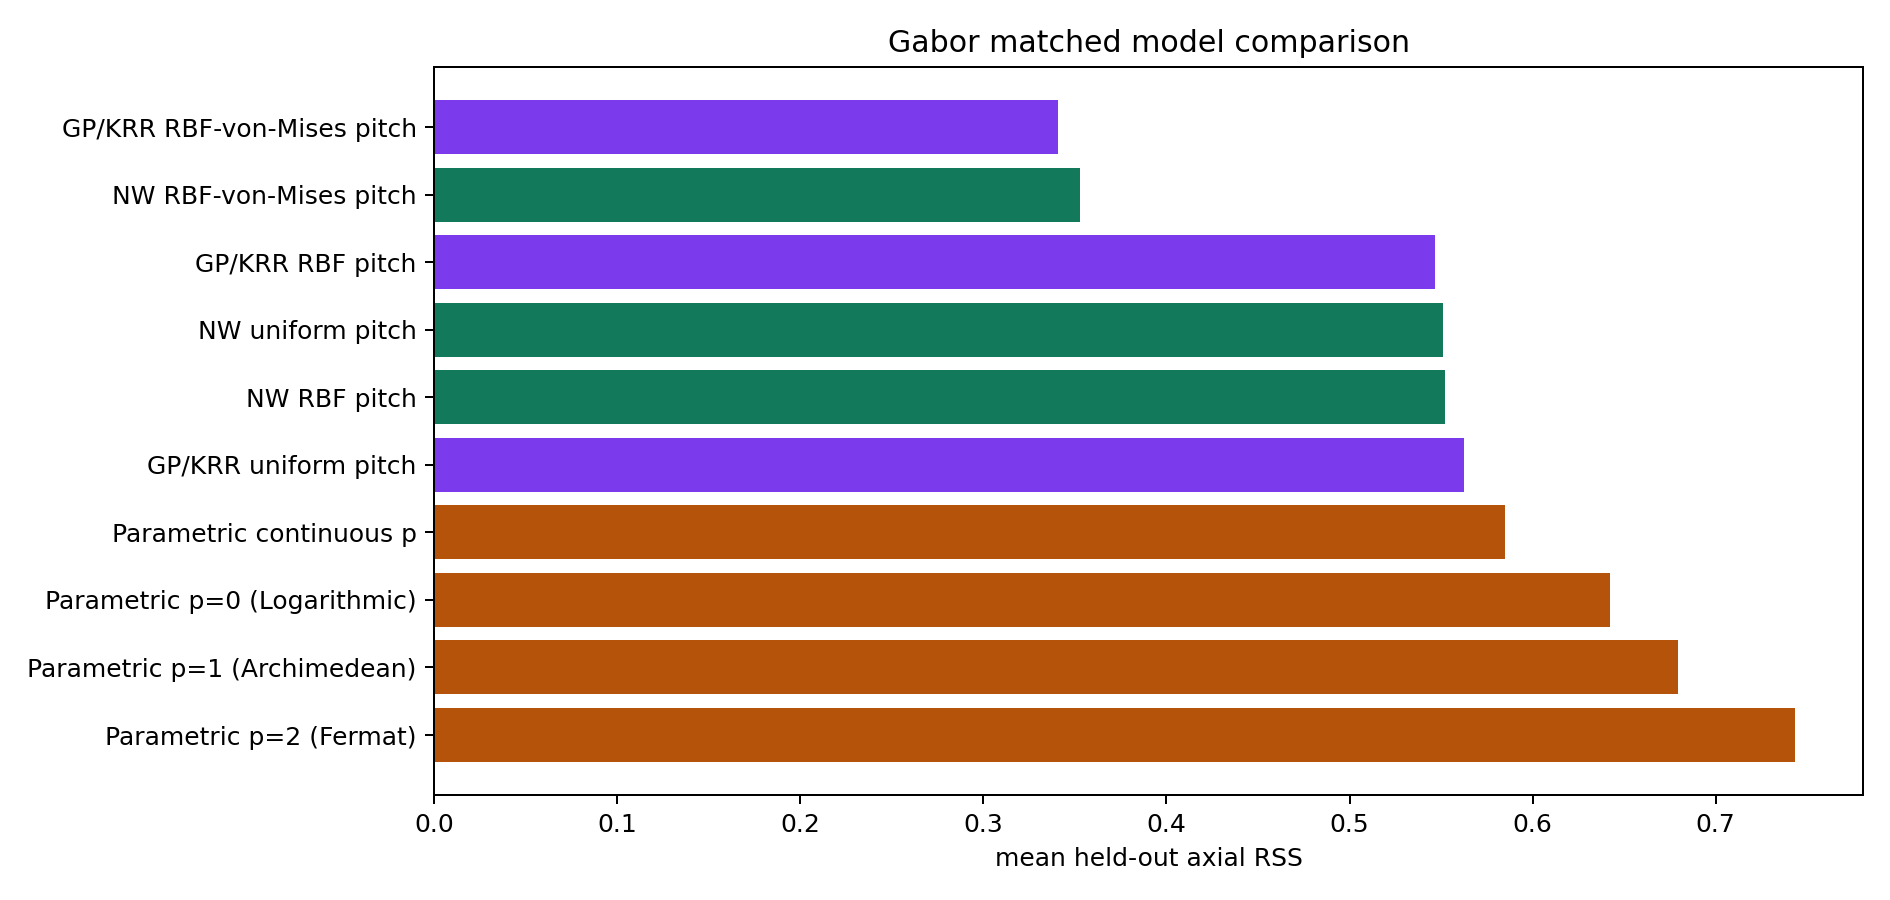
\includegraphics[width=\linewidth]{gabor_nw_gp_mean_rss.png}
\end{minipage}
\hfill
\begin{minipage}{0.48\linewidth}
\centering
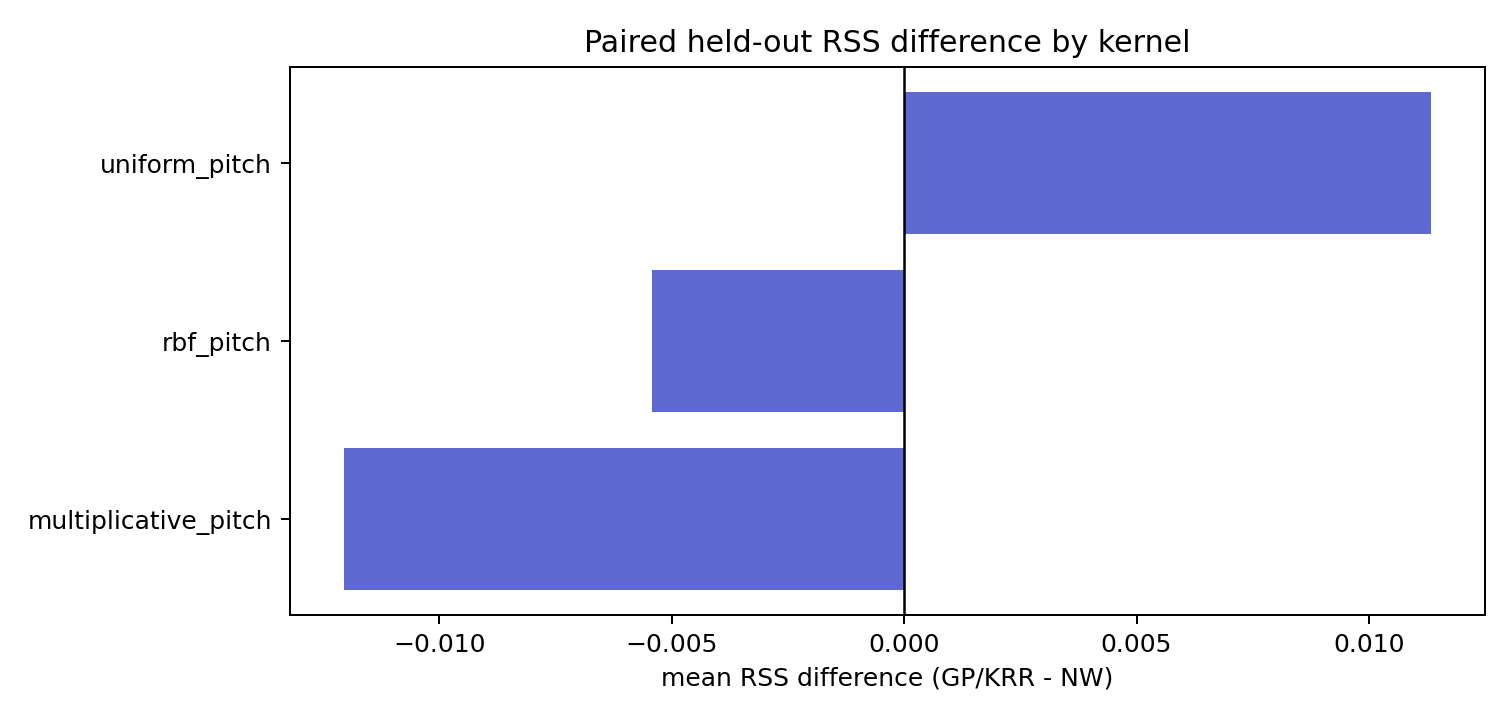
\includegraphics[width=\linewidth]{gabor_gp_minus_nw_rss.png}
\end{minipage}
\caption{Gabor matched NW-versus-GP/KRR summary.  Left: mean held-out RSS.  Right: paired GP/KRR minus NW RSS by kernel; negative values favour GP/KRR.  These score plots should be read together with streamline diagnostics, because the high-$\kappa$ multiplicative model can be visually abrupt despite good held-out RSS.}
\label{fig:gabor-summary}
\end{figure}

\begin{figure}[!htbp]
\centering
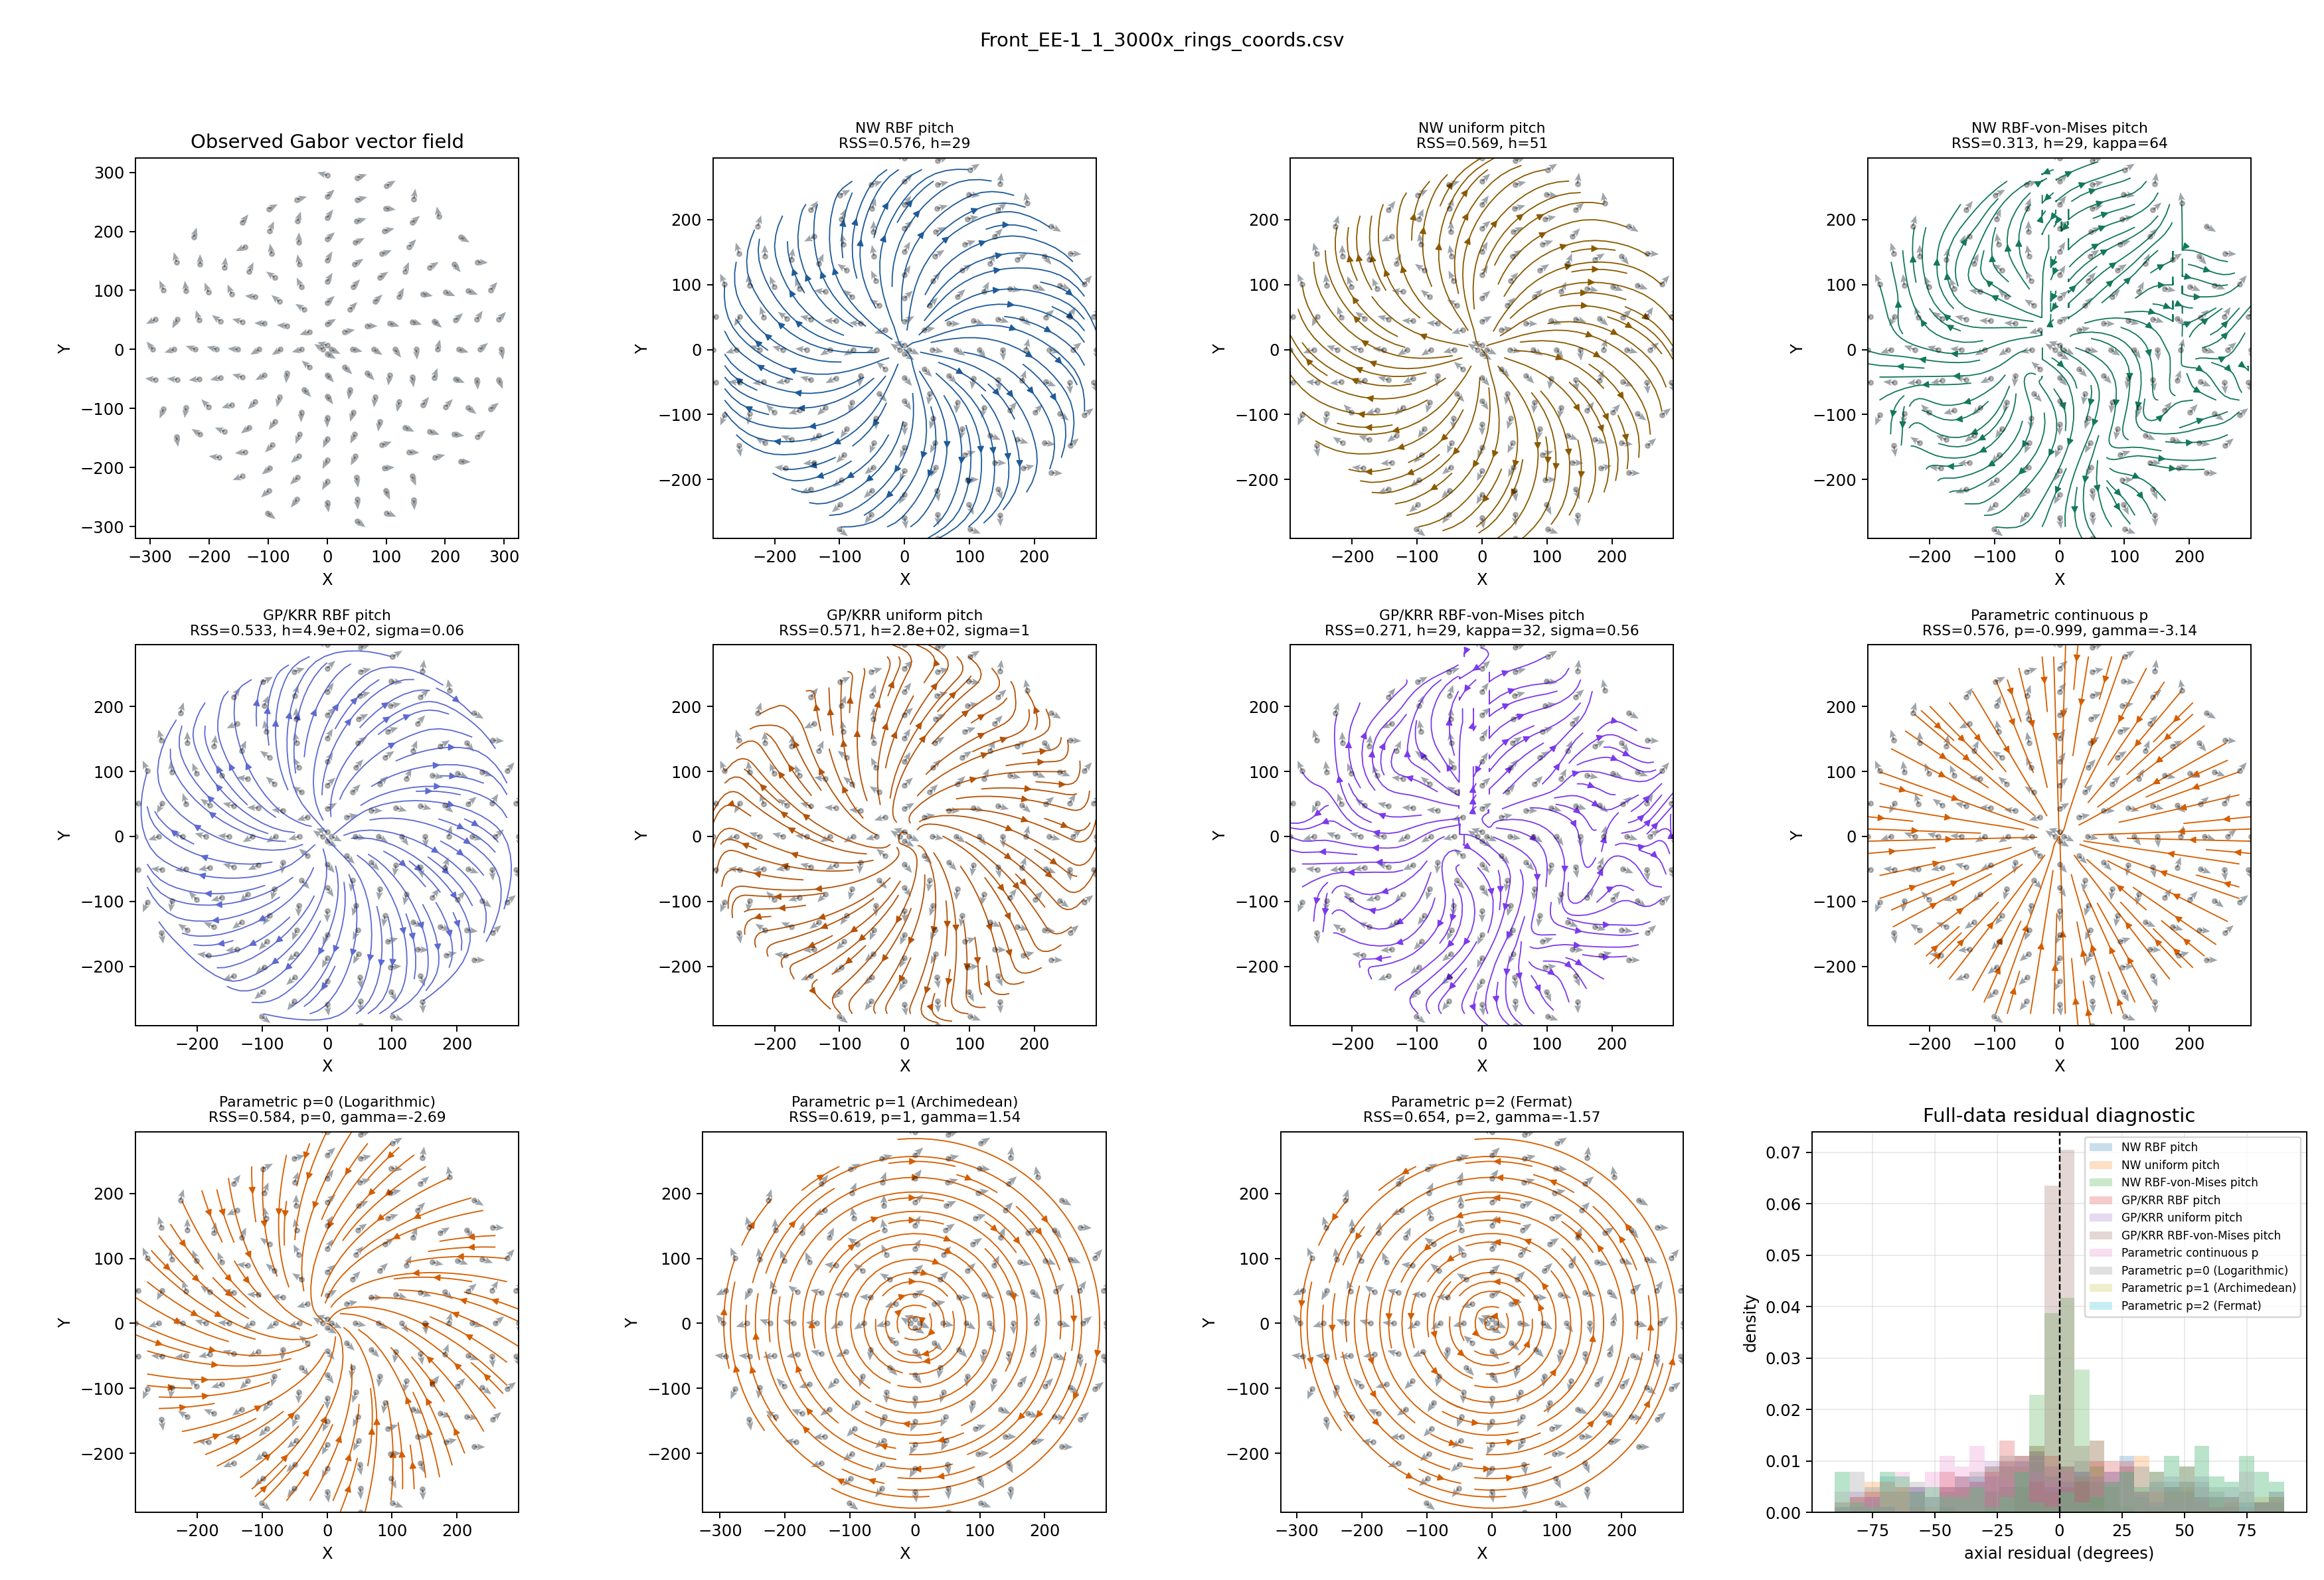
\includegraphics[width=0.92\linewidth]{gabor_nw_gp_streamline_example.png}
\caption{Representative Gabor fitted-field diagnostic from the same matched protocol as Table~\ref{tab:gabor}.  The numerical comparison favours the RBF--von-Mises geometry, but the fitted streamlines are also inspected visually because local angular concentration can introduce abrupt spatial changes.}
\label{fig:gabor-streamline}
\end{figure}

\FloatBarrier
\section{Optical SEM Results}
The optical SEM analysis uses 39 line-field datasets.  These data are not expected to follow one global spiral law, so the parametric family is not the scientific target.  Table~\ref{tab:optical-gp} therefore compares only NW and GP/KRR line-field estimators on the same spatial folds and the same compact kernel grid.  The RBF--von-Mises geometry is again the strongest, and GP/KRR with that kernel has the lowest held-out RSS.

\begin{table}[!htbp]
\centering
\scriptsize
\begin{tabular}{lccc}
\toprule
Model & Mean RSS & Median RSS & Mean MAE \\
\midrule
GP/KRR RBF--von-Mises line field & 0.1422 & 0.1427 & $14.33^\circ$ \\
NW RBF--von-Mises line field & 0.1737 & 0.1519 & $16.55^\circ$ \\
GP/KRR RBF line field & 0.1760 & 0.1646 & $16.16^\circ$ \\
NW RBF line field & 0.2134 & 0.2095 & $19.11^\circ$ \\
NW uniform line field & 0.2273 & 0.2194 & $20.21^\circ$ \\
GP/KRR uniform line field & 0.5345 & 0.5362 & $34.76^\circ$ \\
\bottomrule
\end{tabular}
\caption{Matched optical SEM line-field comparison on the doubled-angle embedding.  Every row uses the same spatial folds and compact kernel grid.}
\label{tab:optical-gp}
\end{table}

The uniform GP/KRR row is poor, reinforcing that a kernel useful for local averaging need not be a good global covariance for matrix inversion.  Thus GP/KRR is justified here only when the chosen kernel is smooth/positive and the fitted streamlines remain visually smooth.

\begin{figure}[!htbp]
\centering
\begin{minipage}{0.48\linewidth}
\centering
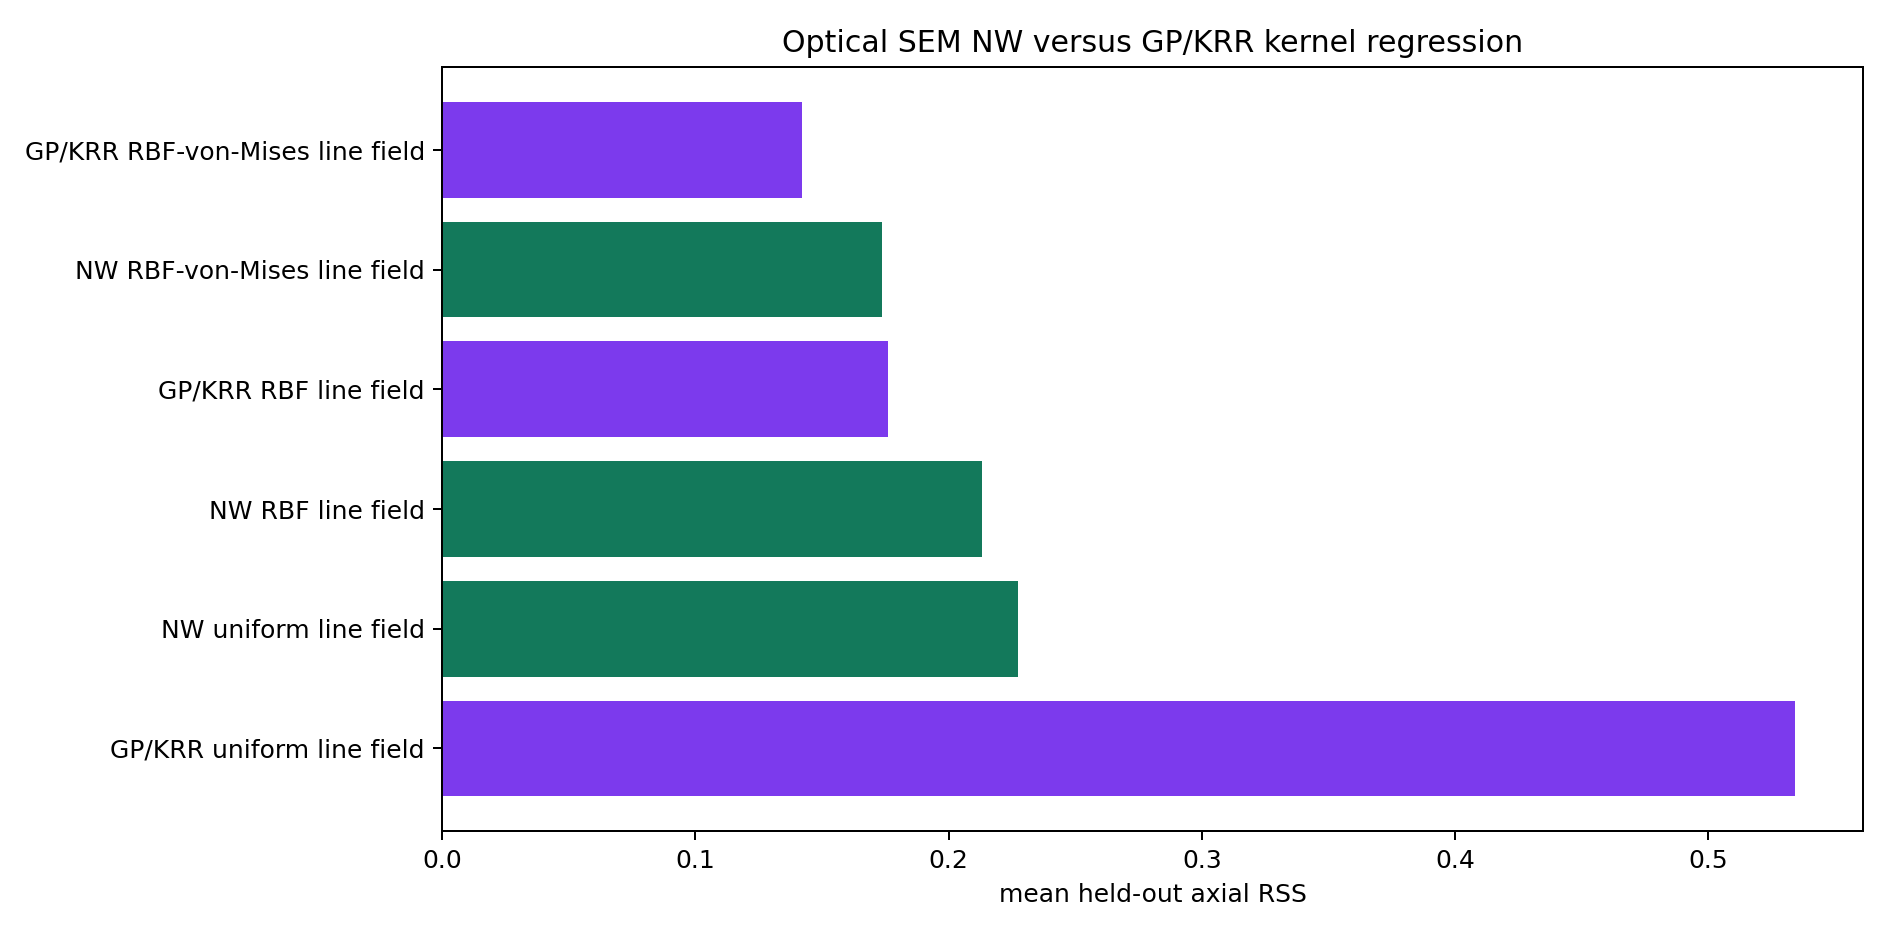
\includegraphics[width=\linewidth]{optical_nw_gp_mean_rss.png}
\end{minipage}
\hfill
\begin{minipage}{0.48\linewidth}
\centering
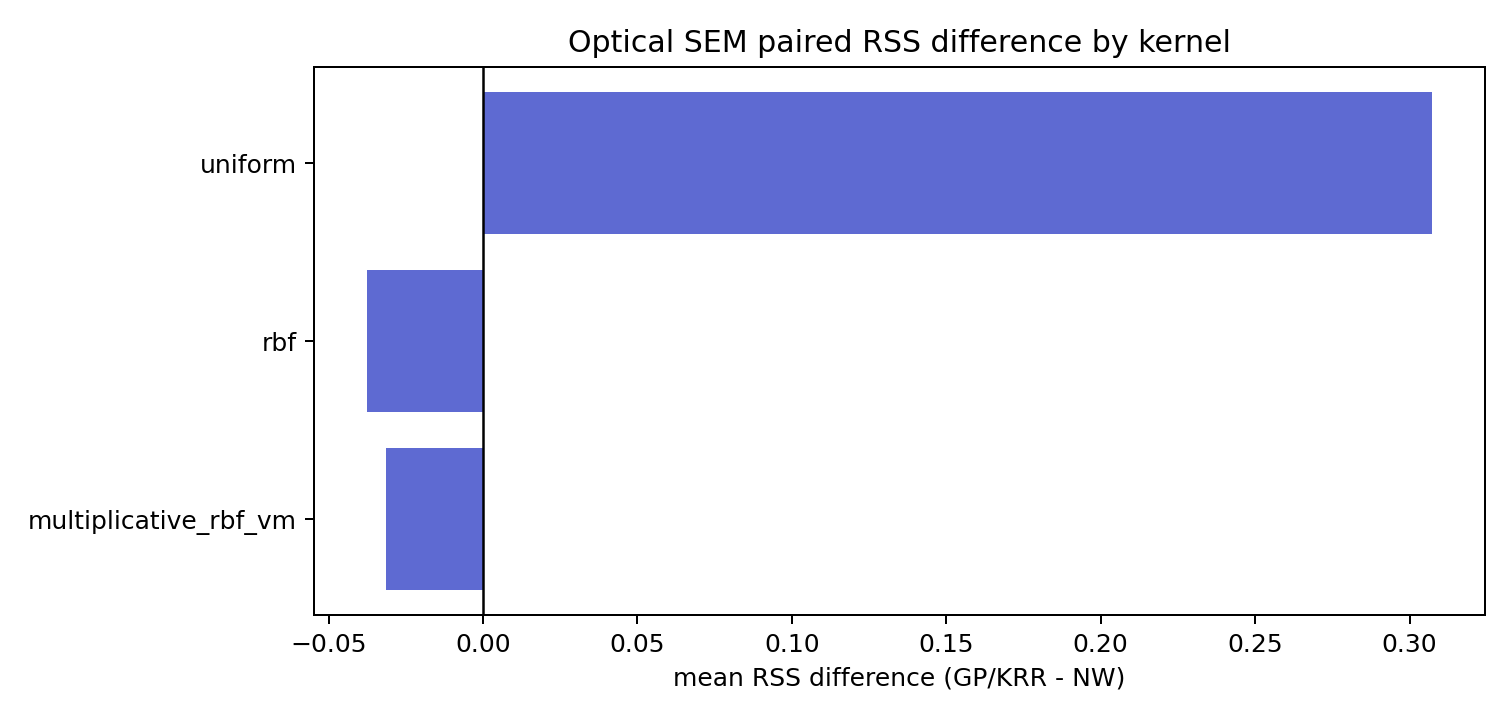
\includegraphics[width=\linewidth]{optical_gp_minus_nw_rss.png}
\end{minipage}
\caption{Optical SEM matched NW-versus-GP/KRR summaries.  Left: mean held-out RSS.  Right: paired GP/KRR minus NW RSS by kernel; negative values favour GP/KRR.}
\label{fig:optical-summary}
\end{figure}

\begin{figure}[!htbp]
\centering
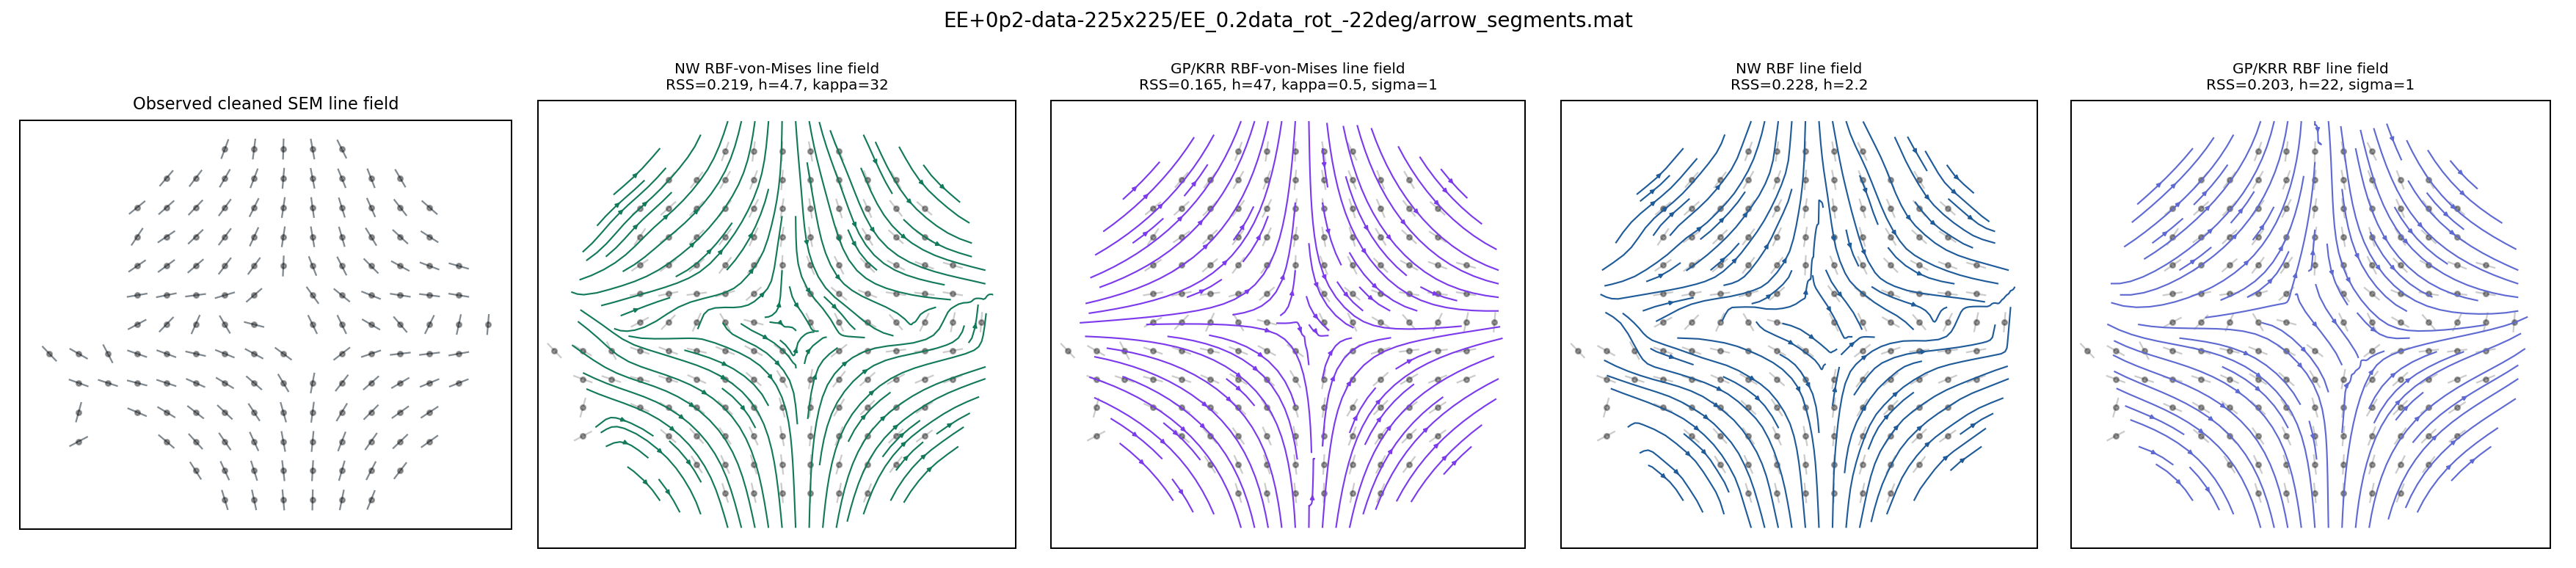
\includegraphics[width=0.92\linewidth]{optical_nw_gp_streamline_example.png}
\caption{Representative optical SEM fitted-field diagnostic from the matched NW/GP-KRR comparison.  This plot complements the held-out RSS table by showing whether the fitted line field follows the observed segment geometry.}
\label{fig:optical-streamline}
\end{figure}

\FloatBarrier
\section{Model-Selection Conclusion}
Let $R(\mathcal M)=\mathbb E\{\Delta^{\rm ax}(\mathcal M)^2\}$ denote axial prediction risk.  Cross-validation estimates this risk and is used here as the model-selection criterion \cite{arlot2010}.  Under the noisy observation model, the parametric class in \eqref{eq:parametric} is a finite-dimensional family for the mean function $m$.  Its variance is small and its interpretation is strong, but its approximation error is large when the field contains spatially varying pitch.  The non-parametric classes reduce this bias by replacing the global spiral mean with a kernel estimator.

The two kernel estimators impose different regularization.  The NW estimator \eqref{eq:nw}, introduced by Nadaraya and Watson \cite{nadaraya1964,watson1964}, is a normalized local average and therefore estimates the conditional mean locally.  Its inductive bias is locality.  The GP/KRR estimator \eqref{eq:gpkrr}, in the standard GP regression framework \cite{rasmussen2006}, solves a global regularized least-squares problem in the RKHS generated by a positive-semidefinite kernel.  Its inductive bias is global covariance smoothness.  Therefore GP/KRR should be preferred only when the kernel is a defensible covariance, the held-out risk decreases on the same folds, and the fitted streamline field remains visually regular.  Otherwise, the lower-variance local NW estimator is the more stable descriptive model.

Under this criterion, the Gabor results reject the global parametric spiral family in favour of the RBF--von-Mises kernel.  GP/KRR gives the smallest matched held-out RSS, but the high-$\kappa$ multiplicative streamline can appear abrupt; that visual diagnostic weakens the case for reporting it as the sole final model.  For optical SEM, the parametric spiral family is not the target model class; the matched kernel comparison again favours the RBF--von-Mises geometry, with GP/KRR improving held-out RSS when the covariance interpretation is defensible.  For multiple particles or repeated vector-field samples, the appropriate extension is to fit per-particle NW diagnostics first and move to pooled or hierarchical GP/KRR only when the samples plausibly share a common latent field.

\bibliographystyle{plain}
\bibliography{references}
\end{document}
